
\section{Methodik}
\subsection{Experimenteller Aufbau}
Der experimentelle Aufbau umfasste drei Gruppen: eine Kontrollgruppe ohne verbale Stimulation, eine Gruppe mit positiver Stimulation und eine Gruppe mit negativer Stimulation. Die Samen wurden unter identischen Wachstumsbedingungen gehalten, außer in Bezug auf die verbale Beeinflussung.

\subsection{Pflege und Bedingungen}
Jede Pflanze wurde alle zwei Tage mit 100 ml Wasser gegossen.

\subsection{Beschallungssystem}
Zur verbalen Stimulation wurden Lautsprecher eingesetzt, die in einem Abstand von etwa 10 - 15 cm zur Pflanze positioniert waren. Die für Beleidigungen und Lob verwendeten Stimmen wurden mit TTSMaker erzeugt (Stimme: "120094 - Kasper Germany Male"). \cite{ttsmaker} Folgende Aussagen wurden für die Beleidigungen verwendet:
\begin{itemize}
    \item "Du bist eine schlechte Pflanze."
    \item "Du bist hässlich."
    \item "Du bist zu dumm zum Wachsen."
\end{itemize}
Für das Lob wurden folgende Aussagen genutzt:
\begin{itemize}
    \item "Du bist wunderschön."
    \item "Du bist eine tolle Pflanze."
    \item "Du bist beeindruckend."
\end{itemize}

\begin{figure} [H]
    \centering
    \begin{minipage}{.37\textwidth}
        \centering
        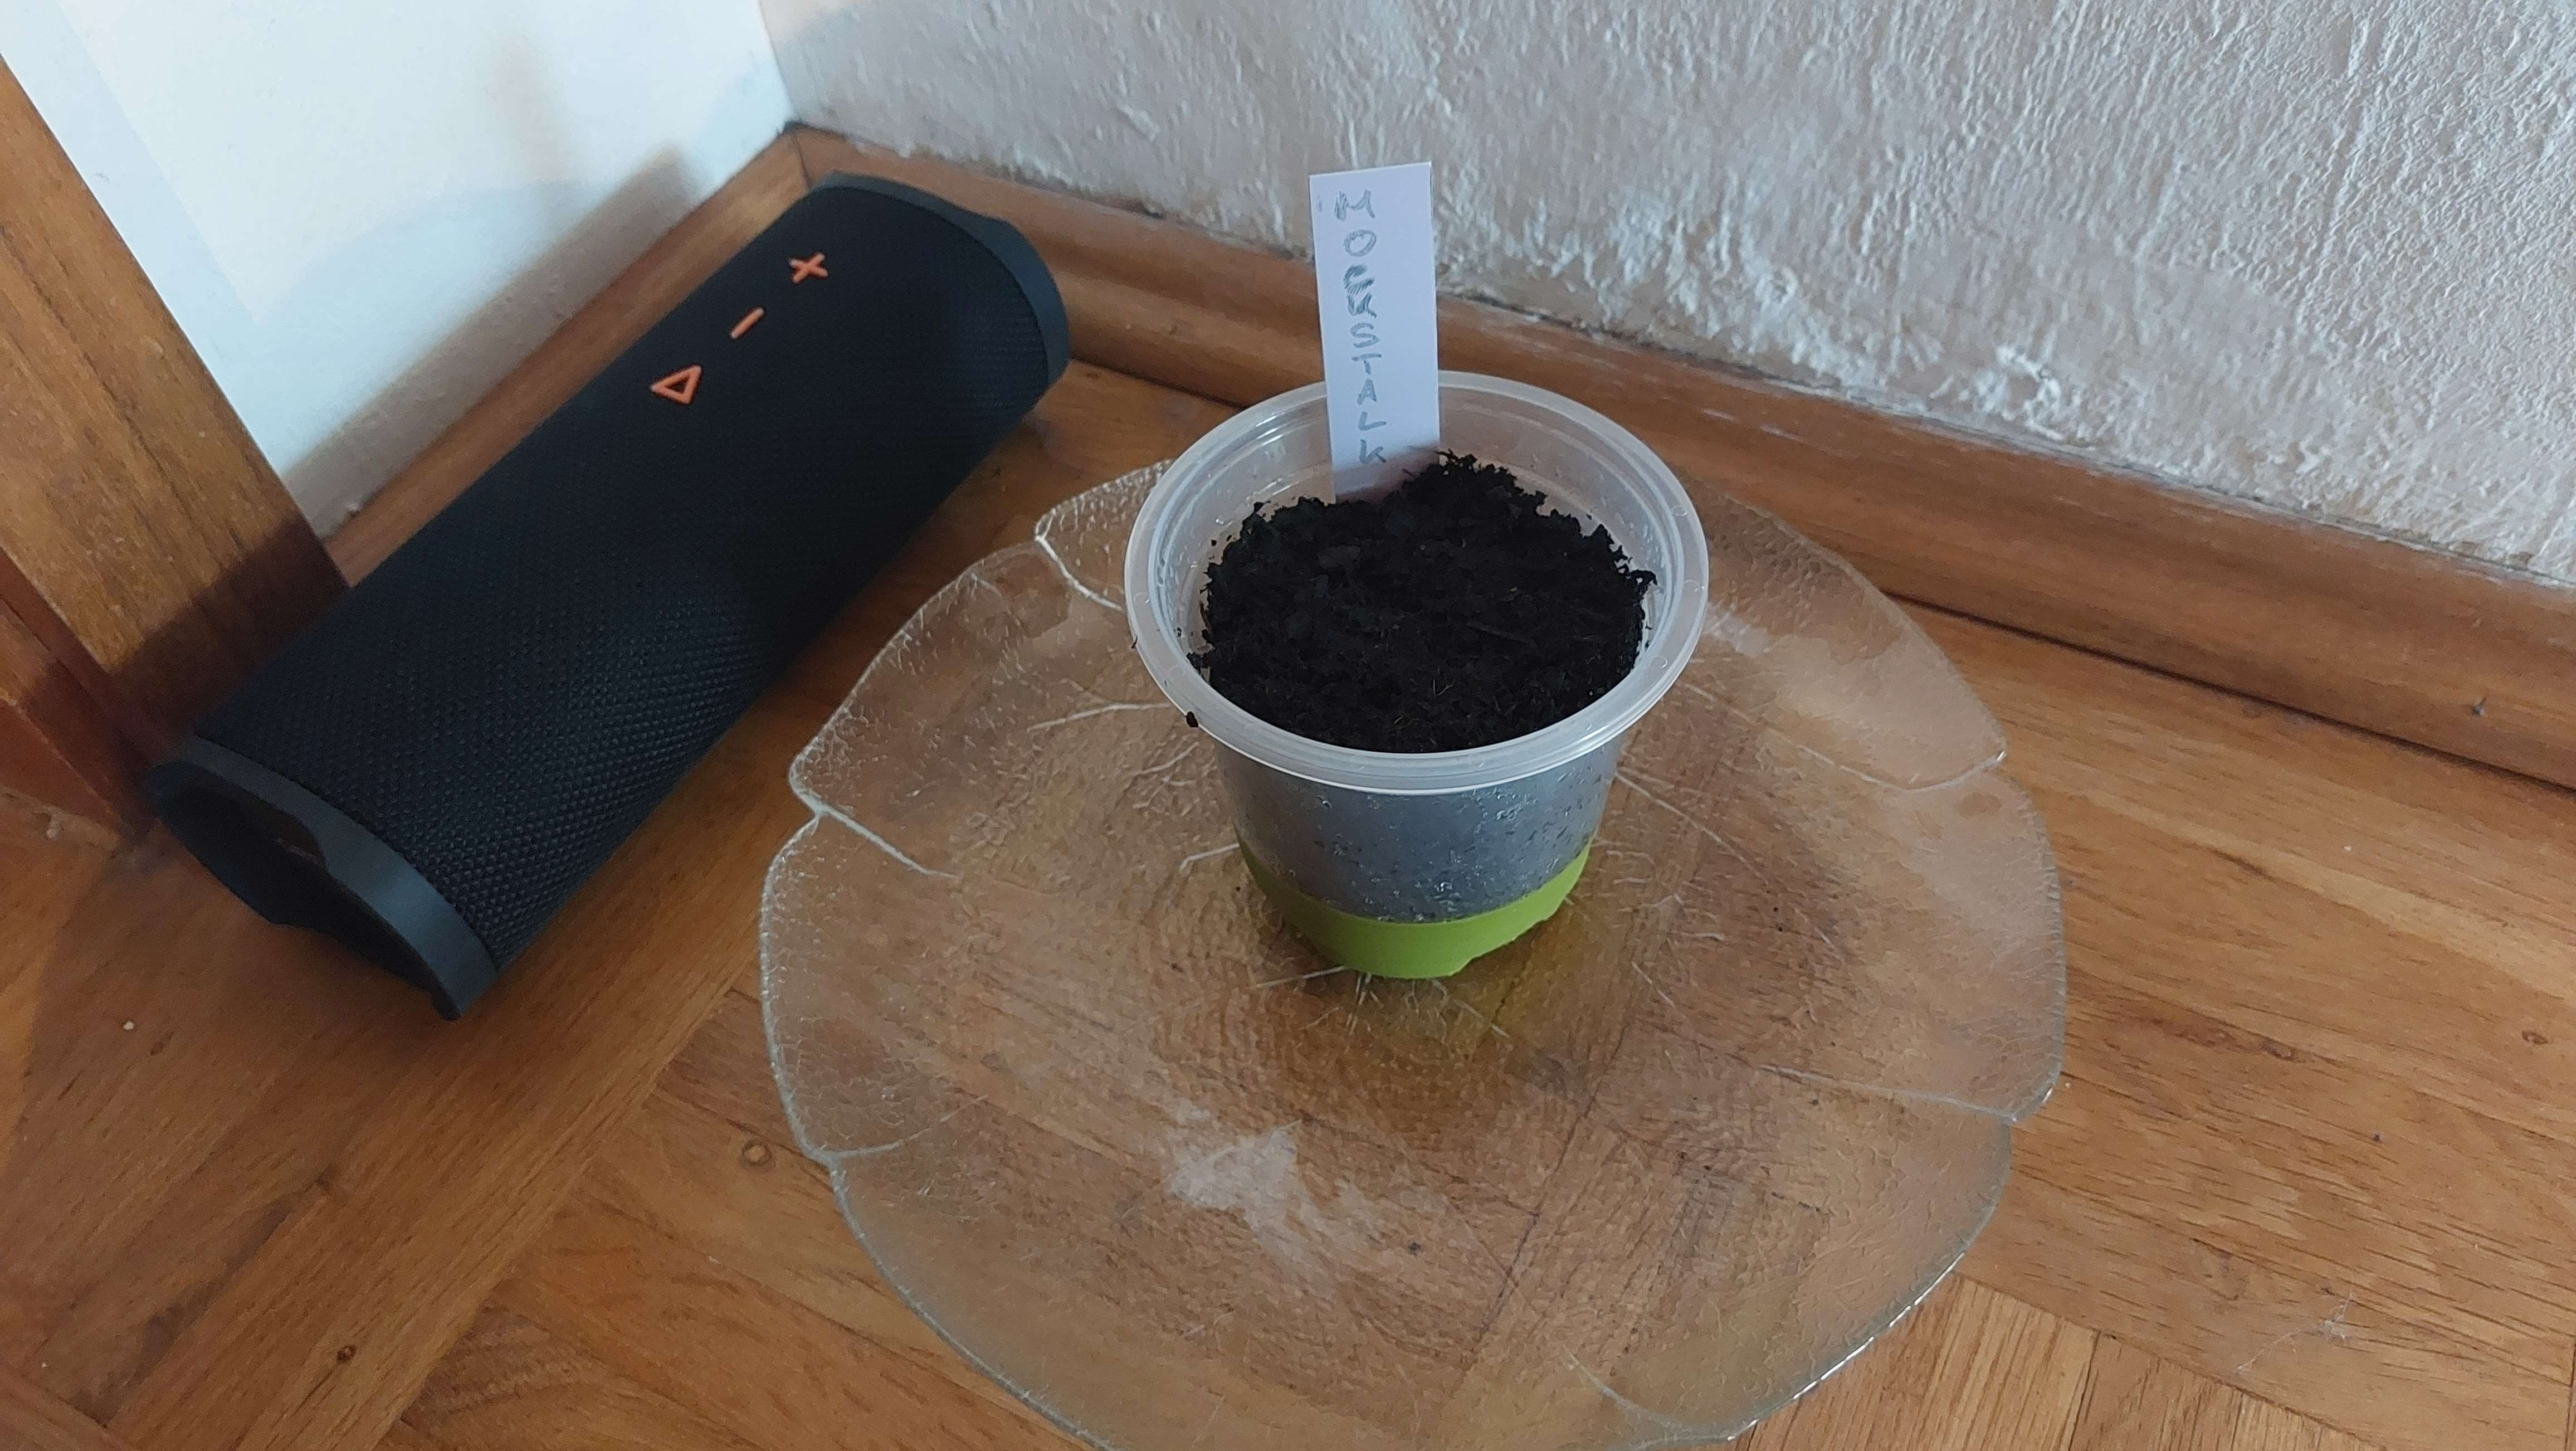
\includegraphics[width=5cm]{Pflanze_schlecht.jpg}
        \caption{Mockstalk}
        \label{fig:schlecht}
    \end{minipage}%
    \begin{minipage}{.37\textwidth}
        \centering
        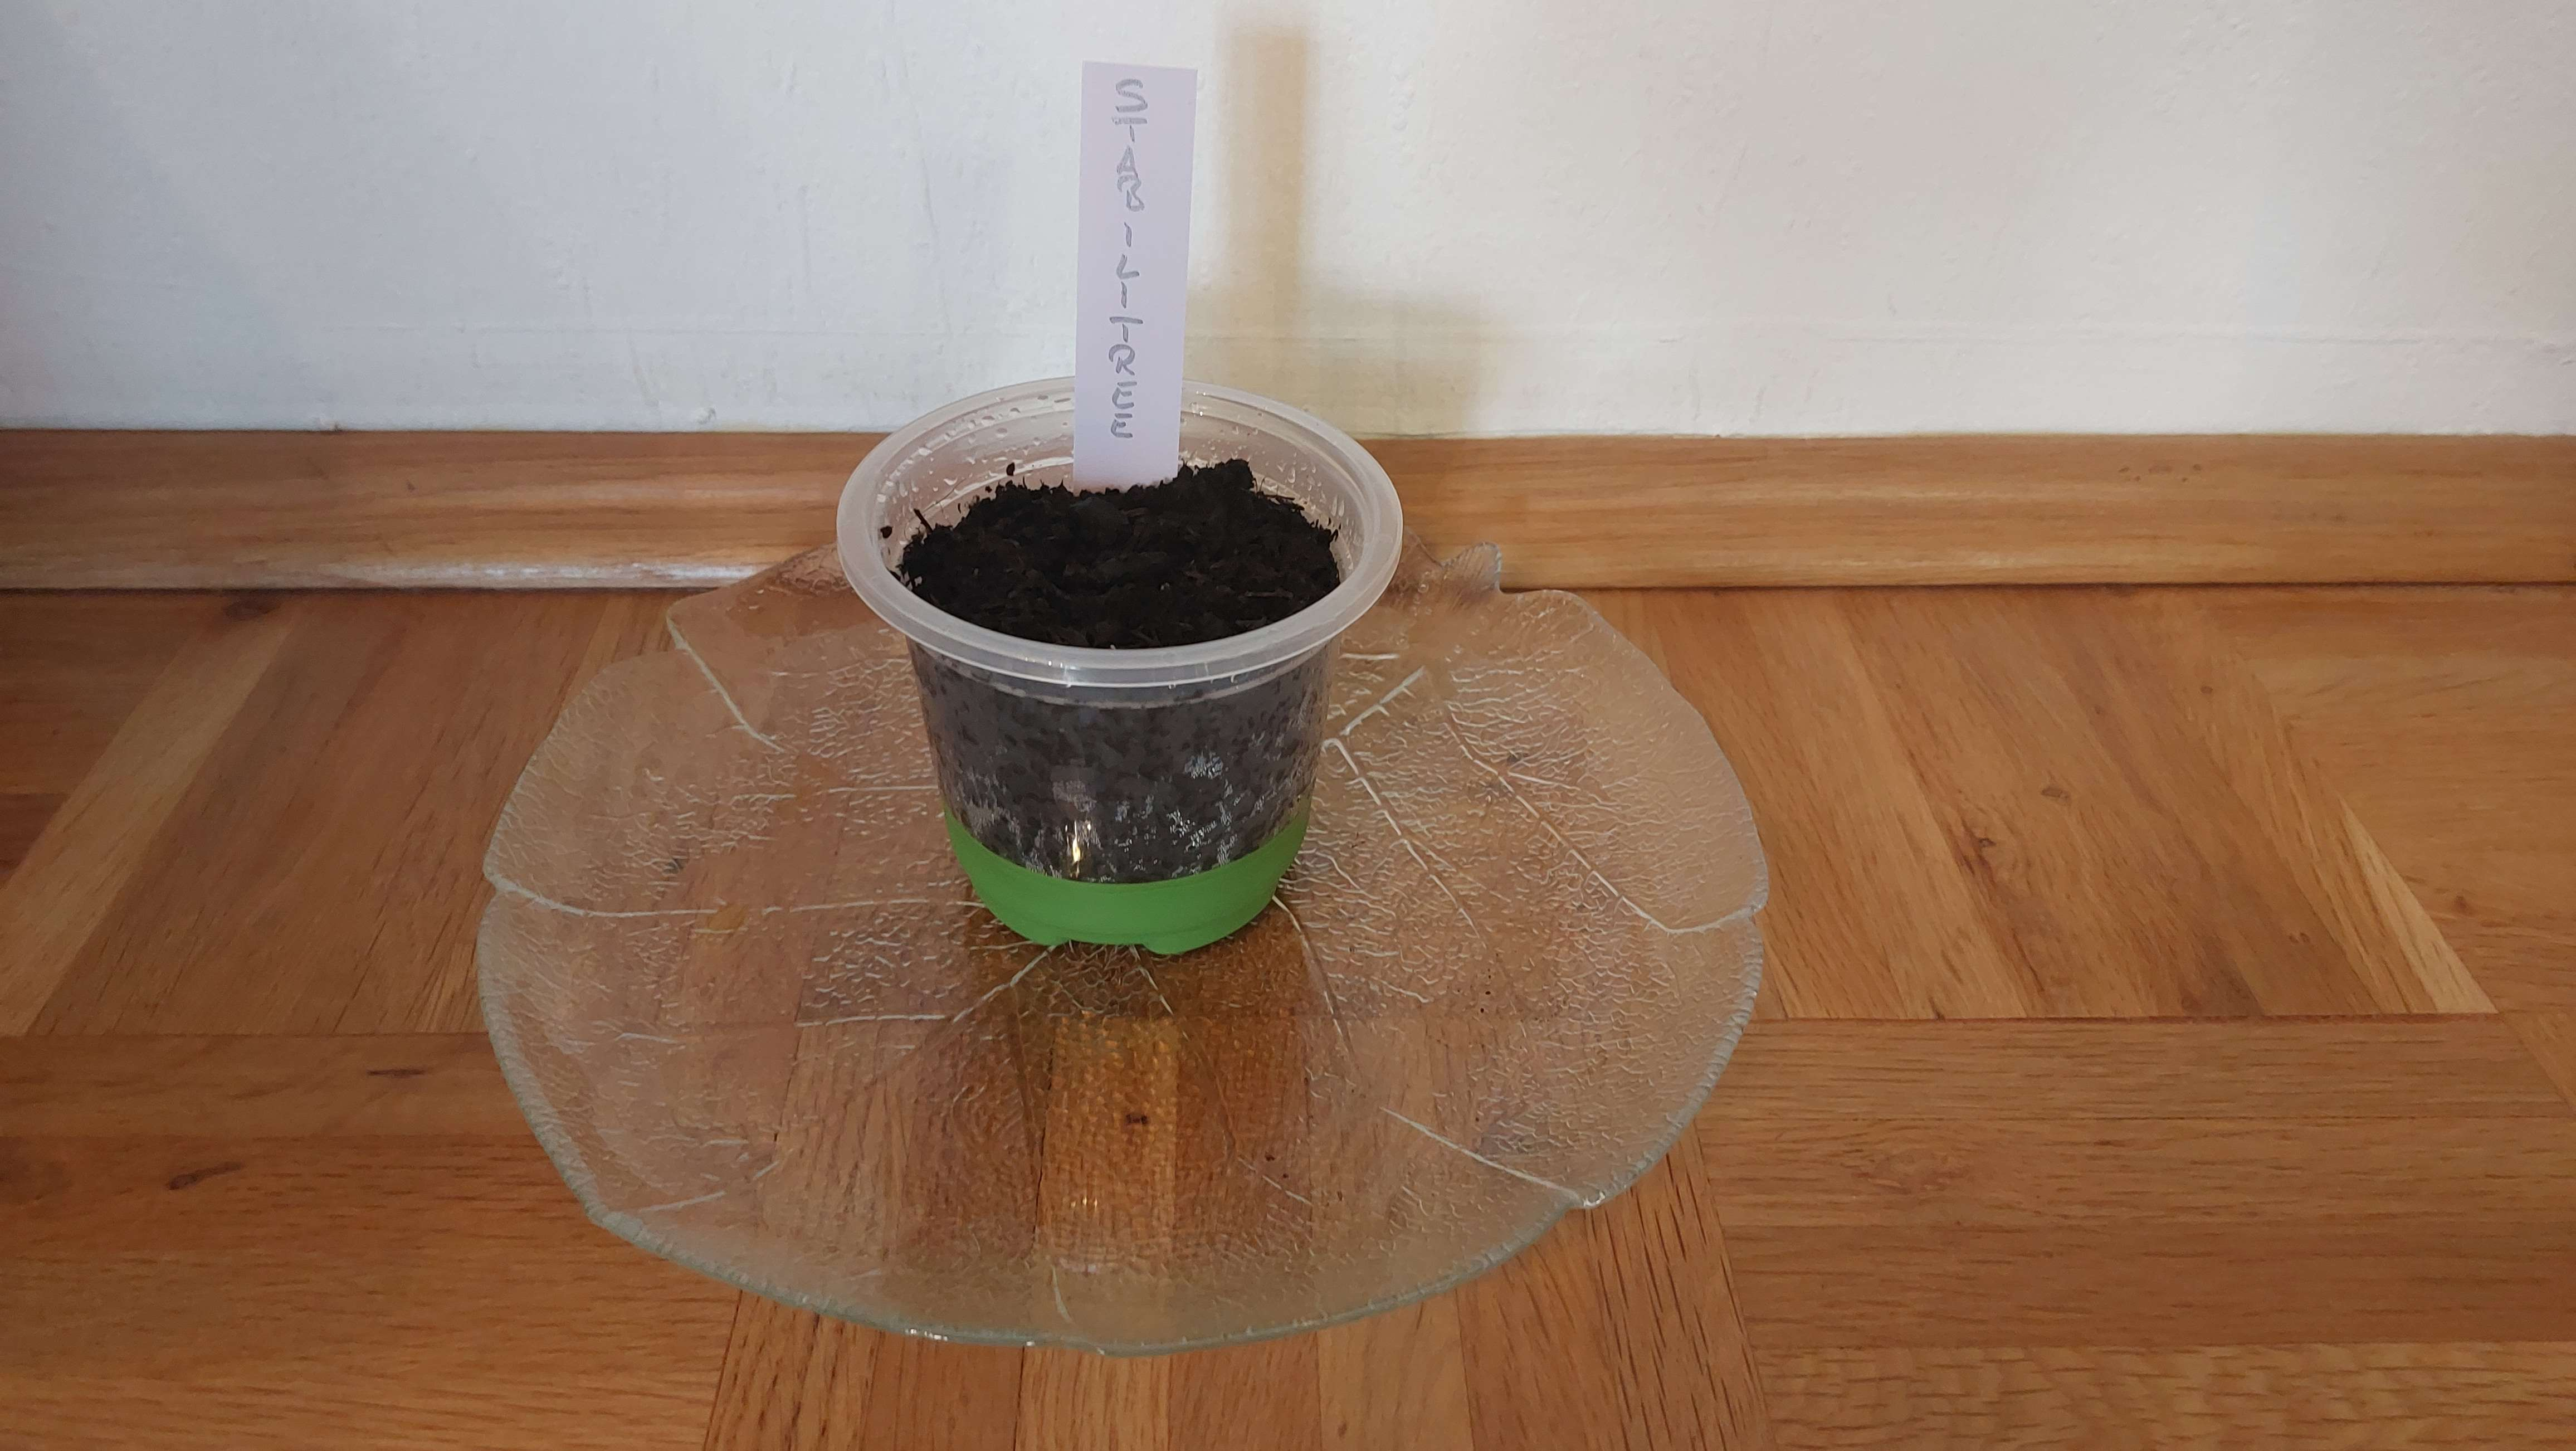
\includegraphics[width=5cm]{Pflanze_normal.jpg}
        \caption{Stabilitree}
        \label{fig:normal}
    \end{minipage}%
    \begin{minipage}{.37\textwidth}
        \centering
        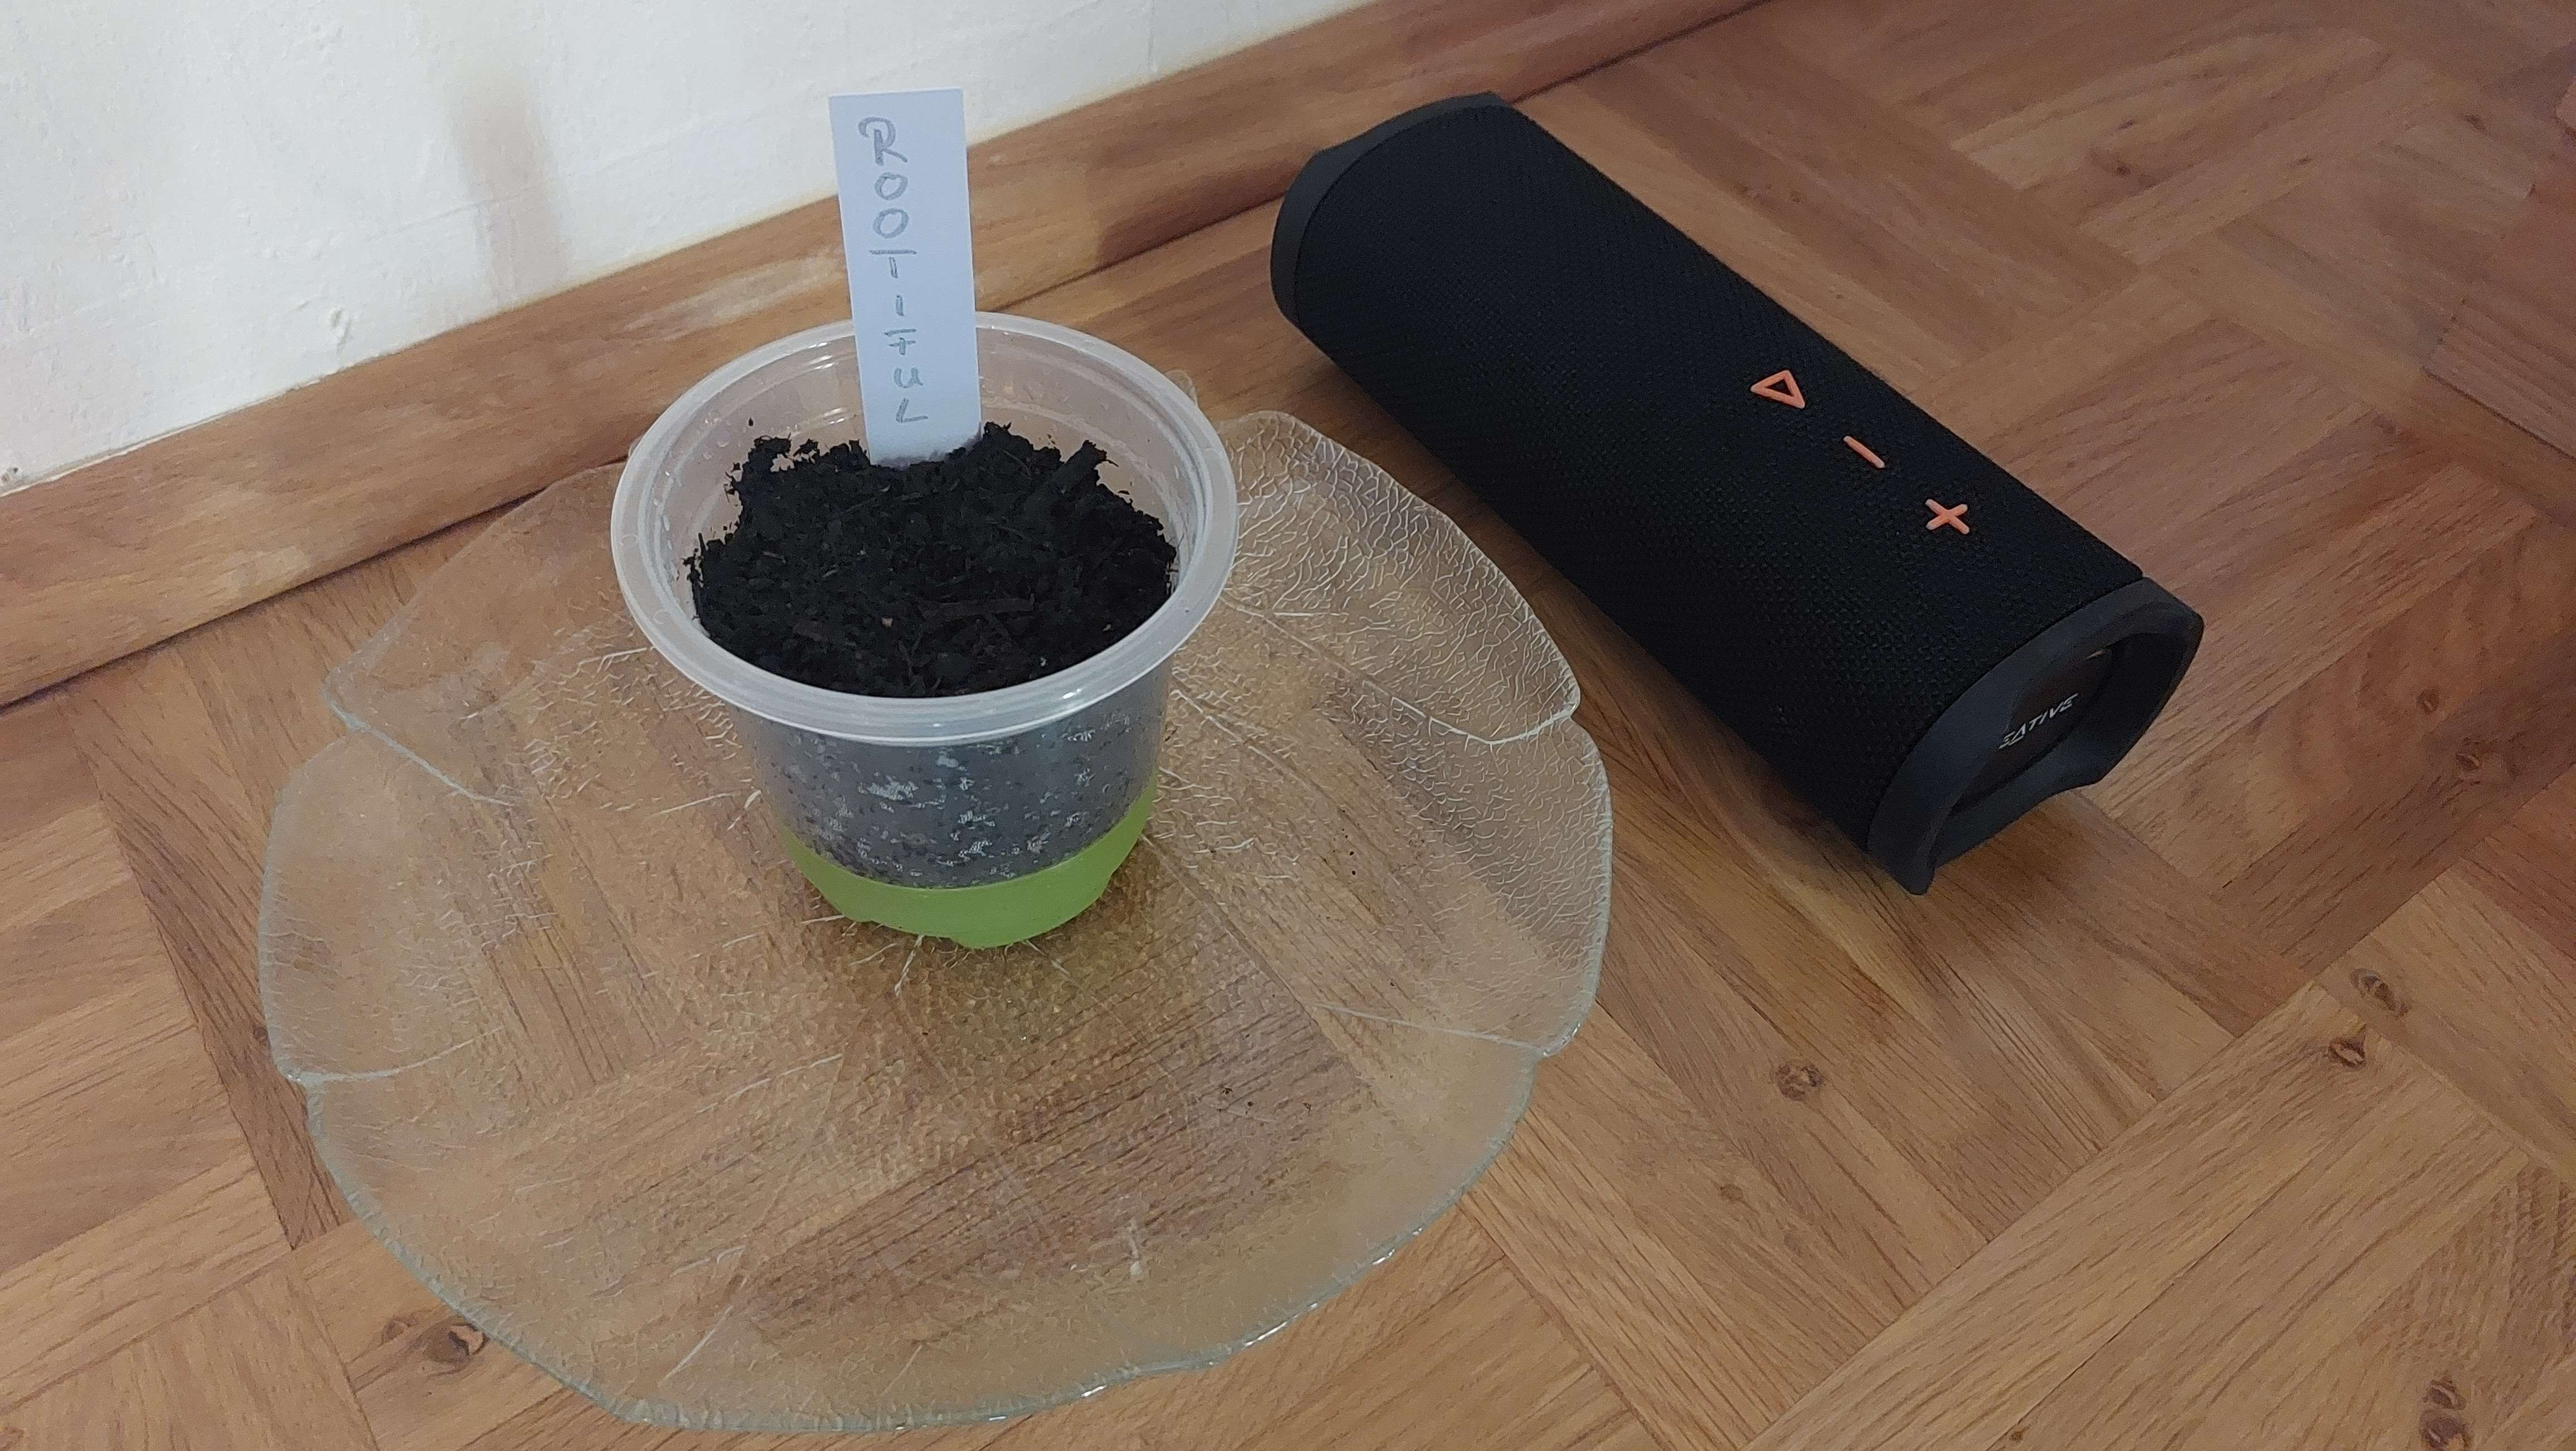
\includegraphics[width=5cm]{Pflanze_lob.jpg}
        \caption{Rootiful}
        \label{fig:gut}
    \end{minipage}
    \label{fig:alle_bilder}
\end{figure}


\subsection{Datenerhebung und Analyse}
Die Entwicklung der Samen wurde über einen Zeitraum von 14 Tagen beobachtet, und Parameter wie die Anzahl und Größe der Sämlinge sowie die Wurzelentwicklung wurden gemessen.

\pagebreak

\section{Ergebnisse}
\subsection{Sprosslinge}
Die Entwicklung der Sprosslinge wurde wie folgt beobachtet:
\begin{itemize}
    \item \textbf{Stabilitree:} Die Samen der Stabilitree waren die einzigen, die eine sichtbare Entwicklung zeigten. Sie begannen zu wachsen und keimten leicht.
    \item \textbf{Rootiful und Mockstalk:} Die Samen in diesen beiden Gruppen zeigten keine sichtbaren Entwicklung.
\end{itemize}

\subsection{Wurzeln}
Die Wurzelentwicklung wurde während des 14-tägigen Beobachtungszeitraums untersucht. Es konnte keine signifikante Wurzelbildung in den Samen festgestellt werden, trotz regelmäßiger Bewässerung und optimalen Wachstumsbedingungen.

\begin{figure} [H]
    \centering
    \centering
    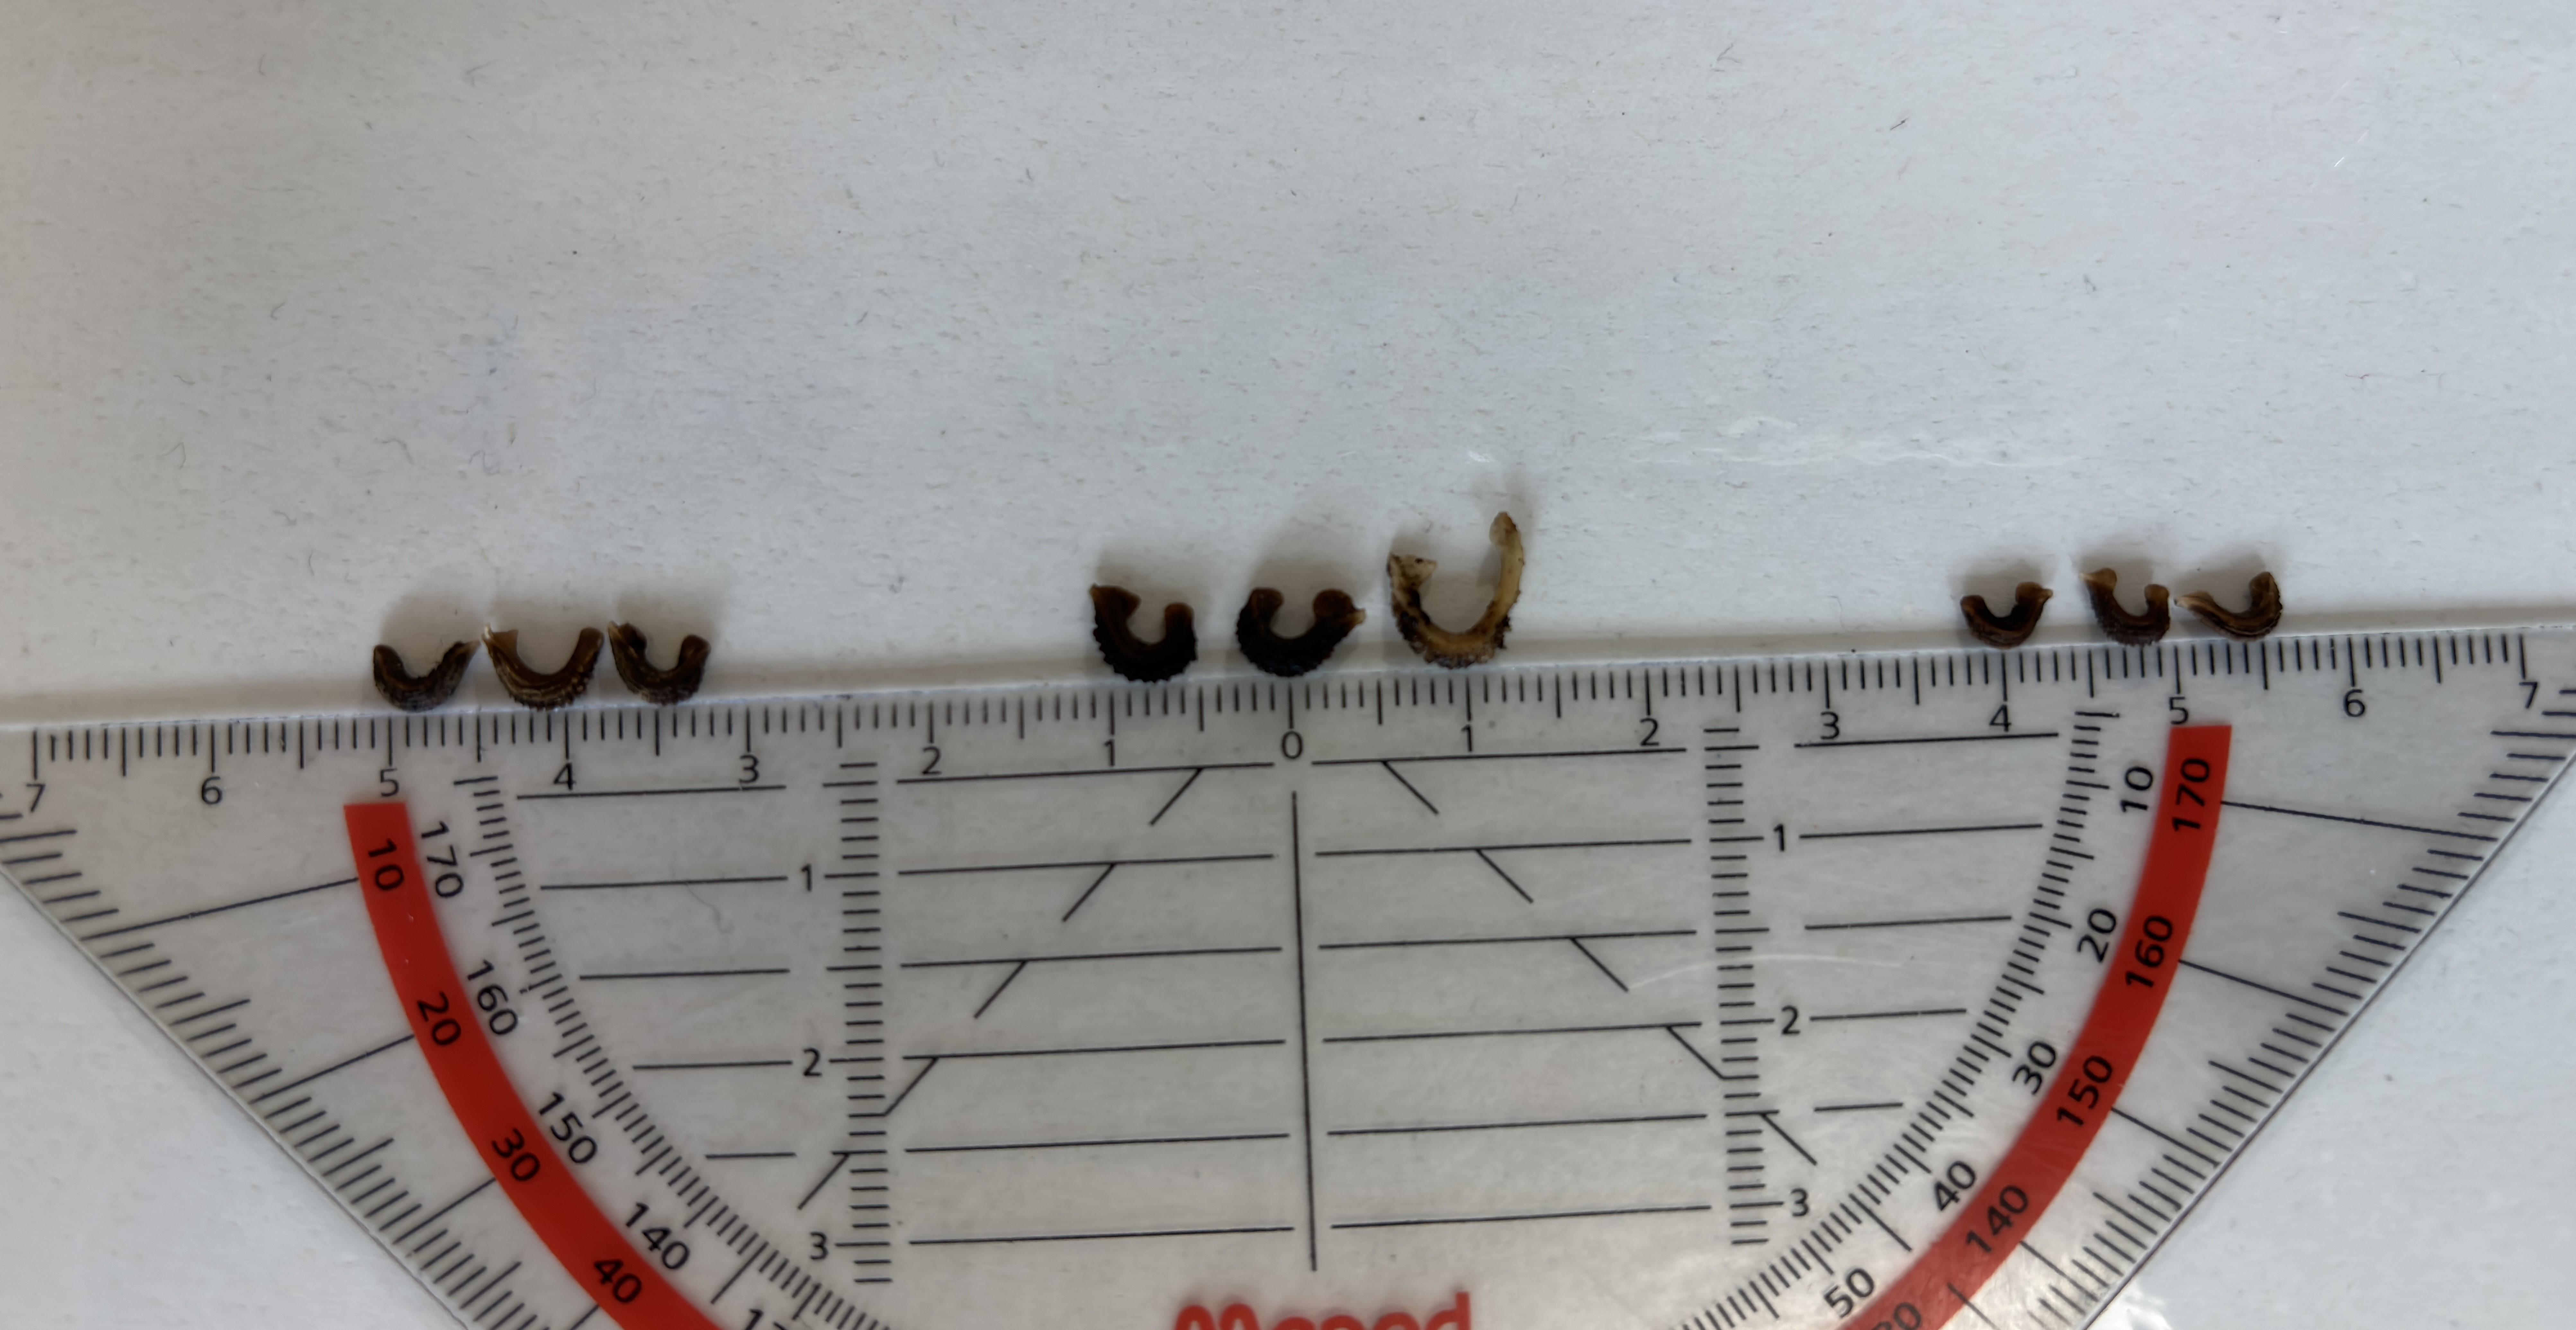
\includegraphics[width=\textwidth]{SamenBild.jpeg}
    \caption{Von links nach rechts: "Rootiful", "Stabilitree", "Mockstalk"}
    \label{fig:enter-label}
\end{figure}

\pagebreak

\section{Diskussion}
\subsection{Interpretation der Ergebnisse}
Die Ergebnisse deuten darauf hin, dass verbale Beeinflussung das Wachstum und die Gesundheit von Pflanzen beeinflussen kann. Die größte Überraschung war, dass die Kontrolle ohne jegliche verbale Stimulation (Stabilitree) die besten Ergebnisse zeigte, was darauf hindeuten könnte, dass Pflanzen unter natürlichen Bedingungen am besten gedeihen. Dies steht jedoch im Widerspruch zu Studien, welche einen positiven Einfluss von verbaler Beeinflussung hervorheben \cite{Yi2003Effect, chowdhury-gupta2015}.

\subsection{Mögliche Erklärungen}
\begin{itemize}
    \item \textbf{Stressfaktoren:} Die Ergebnisse deuten darauf hin, dass künstlich erzeugte Worte als Stressoren wirken können, die das Pflanzenwachstum hemmen. 
    \item \textbf{Beobachtungszeitraum:} Der kurze Beobachtungszeitraum von 14 Tagen war möglicherweise nicht ausreichend, um eine vollständige Wurzelentwicklung zu beobachten. Ein längerer Zeitraum wäre notwendig gewesen, um die Unterschiede in der Wurzelbildung besser beurteilen zu können.
\end{itemize}

\subsection{Limitationen der Studie}
\begin{itemize}
    \item \textbf{Kleine Stichprobengröße:} Die begrenzte Anzahl von Samen (jeweils 5 Samen) reduziert die statistische Aussagekraft.
    \item \textbf{Kurzer Beobachtungszeitraum:} Die Durchführung des Experiments über nur 14 Tage war möglicherweise zu kurz, um die vollständigen Auswirkungen der verbalen Beeinflussung auf die Samenentwicklung zu erfassen. Ein längerer Zeitraum wäre wünschenswert gewesen, insbesondere um die Wurzelentwicklung zu beobachten.
\end{itemize}

\subsection{Weitere Forschung}
Zukünftige Studien sollten eine größere Stichprobengröße und einen längeren Beobachtungszeitraum umfassen, um die Ergebnisse zu verifizieren und besser zu verstehen, wie Samen auf verbale Stimulation reagieren. Zusätzlich könnten verschiedene Pflanzenarten und variierende Formen der akustischen Beeinflussung untersucht werden.

\pagebreak

\section{Schlussfolgerung}
Die Studie weist keine Signifikanz auf, weshalb keine Schlussfolgerungen über die Auswirkungen positiver oder negativer verbalen Beeinflussung auf das Wachstum von Pflanzen gezogen werden können. Weder die positiv noch die negativ angesprochenen Samen zeigten signifikante Unterschiede in ihrem Verhalten; beide Gruppen schnitten ähnlich schlecht ab. Einzig die Samen in der "Stabilitree"-Gruppe entwickelten sich positiv und zeigten das stärkste Keimwachstum.  Es wird deutlich gemacht, dass die begrenzte Dauer des Experiments eine wesentliche Einschränkung darstellt, und zukünftige Studien sollten darauf abzielen, umfassendere Beobachtungen und Analysen der Wurzelentwicklung durchzuführen.

